\hypertarget{quickstart-on-crazyflie-drone-positioning-using-the-lighthouse-positioning-system}{%
\section{Quickstart on Crazyflie drone positioning using the lighthouse
positioning
system}\label{quickstart-on-crazyflie-drone-positioning-using-the-lighthouse-positioning-system}}

This documentation is meant to get you up and running with the
lighthouse positioning system with the crazyflie.

Requirements:

Setup:

\begin{itemize}
\tightlist
\item
  A computer with Steam VR and a VIVE headset (only for setup)
\item
  Git
\end{itemize}

Flying:

\begin{itemize}
\tightlist
\item
  A crazyflie radio
\item
  A computer with python 3 and make installed
\item
  An Xbox, PS4, etc. controller (for manual flight with position assist)
\item
  An HTC vive controller (for flying using the grab example)
\end{itemize}

\hypertarget{setup.}{%
\subsection{Setup.}\label{setup.}}

This sets up a crazyflie to a paricular pair of lighthouses. If you want
to pair the crazyflie to another pair of lighthouses or crazyflie, this
phase must be repeated.

\hypertarget{finding-the-origin}{%
\subsubsection{Finding the origin}\label{finding-the-origin}}

The blank scene provided by SteamVR shows the position of the origin
using a series of lines and circles through the headset

\hypertarget{setting-the-origin}{%
\subsubsection{Setting the origin}\label{setting-the-origin}}

The step of setting the origin is not neccesary, but it may be worth
moving it to the centre of the play area as the drone will take off from
this point. We mark the origin and axes with tape.

To set the origin of a lighthouse system. Get a computer and connect the
headset to it. Open Steam VR on the computer (Steam VR is a tool that
can be downloaded from steam).

Navigate to STEAMVR -\textgreater{} Developer -\textgreater{} Developer
Settings 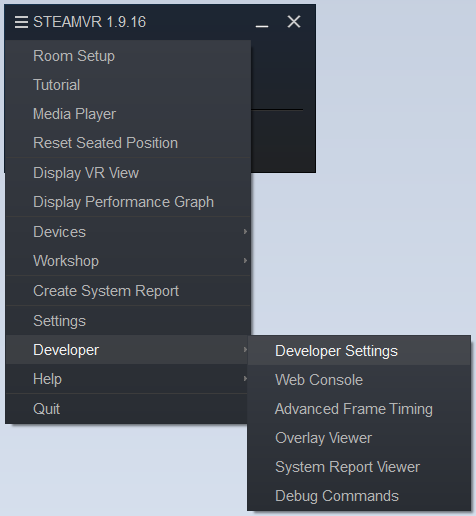
\includegraphics{images/devSettingsPath.png}

Place the headset on the ground in the position you want your origin,
and the direction that you want your positive X to be. The positive Y
will go to the right of the headset and positive Z will go up.

Once the headset is placed press `Quick Calibrate' to set the origin to
the new position. 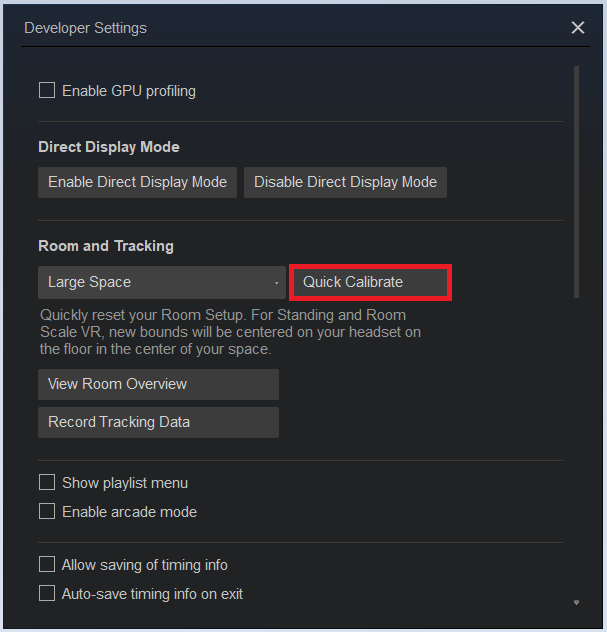
\includegraphics{images/quickCalibrate.png}

\hypertarget{encoding-the-position-of-the-lighthouses-into-the-crazyflie-firmware}{%
\subsubsection{Encoding the position of the lighthouses into the
crazyflie
firmware}\label{encoding-the-position-of-the-lighthouses-into-the-crazyflie-firmware}}

Keep Steam VR running, and do the following on the computer with Steam
VR

To find the position of the lighthouse, check out a copy of the
crazyflie firmware

https://github.com/bitcraze/crazyflie-firmware

Then with python 3. Install openvr and numpy. Then run the script found
in

\begin{verbatim}
crazyflie-firmware/tools/lighthouse/get_bs_position.py
\end{verbatim}

This will give an output that look like this:

\begin{verbatim}
Openning OpenVR
OpenVR Oppened
Origin: {} [0, 0, 0]
-------------------------------
{.origin = {-1.421995, 2.188835, -1.382714, }, .mat = {{-0.773449, 0.339506, -0.535269, }, {0.027097, 0.861399, 0.507206, }, {0.633280, 0.377794, -0.675447, }, }},
{.origin = {1.311097, 2.224771, 1.318952, }, .mat = {{0.641178, -0.457615, 0.616019, }, {0.029892, 0.817028, 0.575823, }, {-0.766810, -0.350791, 0.537539, }, }},
\end{verbatim}

The last 2 lines here are positions and rotations that can be copied
into the firmware for the lighthouse deck.

Copy the results there, and paste them into

\begin{verbatim}
crazyflie-firmare/src/deck/drivers/src/lighthouse.c
\end{verbatim}

inside the lighthouseBaseStationsGeometry variable.

Also, make sure you comment out the \texttt{DISABLE\_LIGHTHOUSE\_DRIVER}
lines before it

\begin{verbatim}
//#ifndef DISABLE_LIGHTHOUSE_DRIVER
//  #define DISABLE_LIGHTHOUSE_DRIVER 1
//#endif
\end{verbatim}

To enable the driver.

Additional details can be found
\href{https://wiki.bitcraze.io/doc:lighthouse:setup}{here}.

\hypertarget{flashing-the-firmware}{%
\subsubsection{Flashing the firmware}\label{flashing-the-firmware}}

The simplest way to build and flash the updated firmware is to use the
CrazyFlie Development VM

https://www.bitcraze.io/getting-started-with-the-crazyflie-2-0/\#inst-virtualmachine

Transfer the firmware to the VM and compile the driver with
\texttt{make}. Then, with the crazyflie radio connected and the
crazyflie booted into firmware mode, run \texttt{make\ cload} to flash
the firmware onto the drone.

\hypertarget{testing-the-setup.}{%
\subsection{Testing the setup.}\label{testing-the-setup.}}

There are several ways to test the setup. As the crazyflie can fly in
unexpected ways if it is not set up correctly, we recommend being fairly
certain that the system works before flying.

\hypertarget{native-vs-vm-client}{%
\subsubsection{Native vs VM client}\label{native-vs-vm-client}}

Flying the drones using the VM client has been known to have issues
during flight. If the VM isn't reliably controling the Crazyflies, try
running the client natively.

https://www.bitcraze.io/getting-started-with-the-crazyflie-2-0/\#installation-flavour

\hypertarget{checking-the-telemetry}{%
\subsubsection{Checking the telemetry}\label{checking-the-telemetry}}

The first thing to do is to start the crazyflie, with the lighthouse
module installed on top of it, within the play space. Make sure that
nobody or nothing is obstructing the crazyflie's view of the two
lighthouses.

Then connect to the crazyflie with the crazyflie client. Make sure that
you have the Look at the logs of the crazyflie. If you are getting
errors such as ``State out of bounds, resetting'' continously or it does
not say that it is ready to fly, then it has not been set up correctly,
and we recommend that you check through the above steps (particularly
commenting out \texttt{DISABLE\_LIGHTHOUSE\_DRIVER}). If the drone says
it is ready to fly, then continue onto the next test.

\begin{figure}
\centering
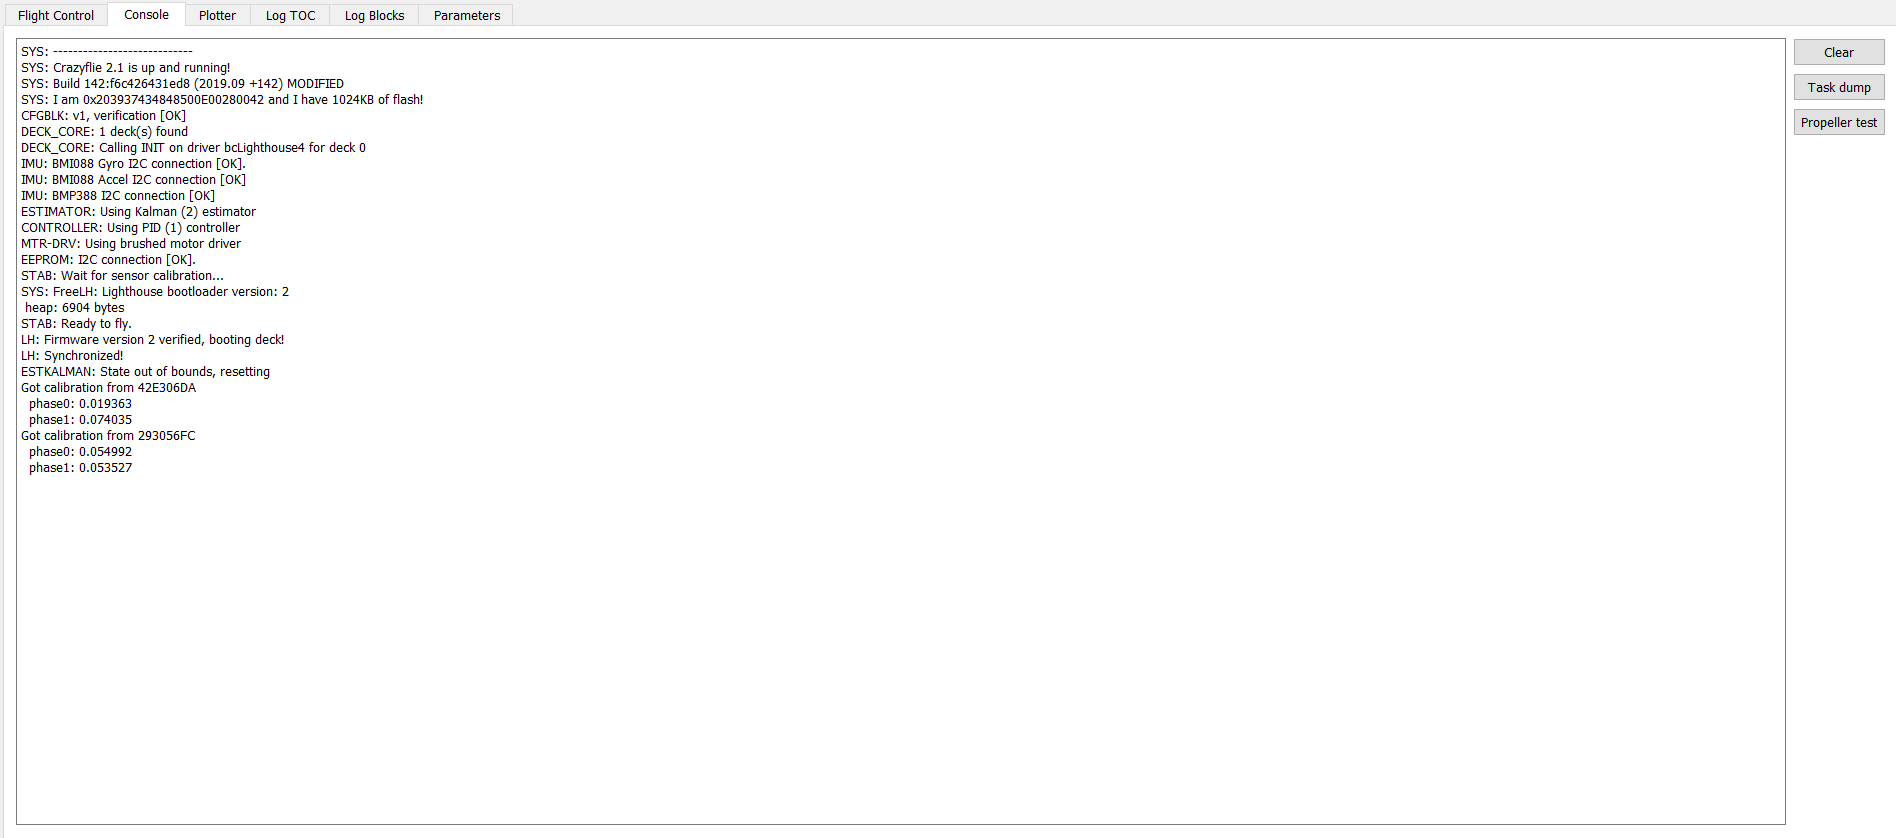
\includegraphics{images/console.png}
\caption{Console}
\end{figure}

\hypertarget{plotting-position-data}{%
\subsubsection{Plotting position data}\label{plotting-position-data}}

The position calculated by the Crazyflie can be plotted by creating a
log block within the client.

To create a log block, connect to the Crazyflie, then open the logging
configuration window.

\begin{figure}
\centering
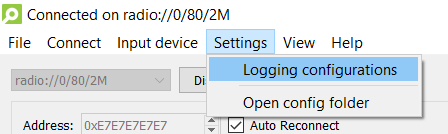
\includegraphics{images/logConfigMenu.png}
\caption{Logging Window Path}
\end{figure}

Fill out the window as shown, then save the new log block.

\begin{figure}
\centering
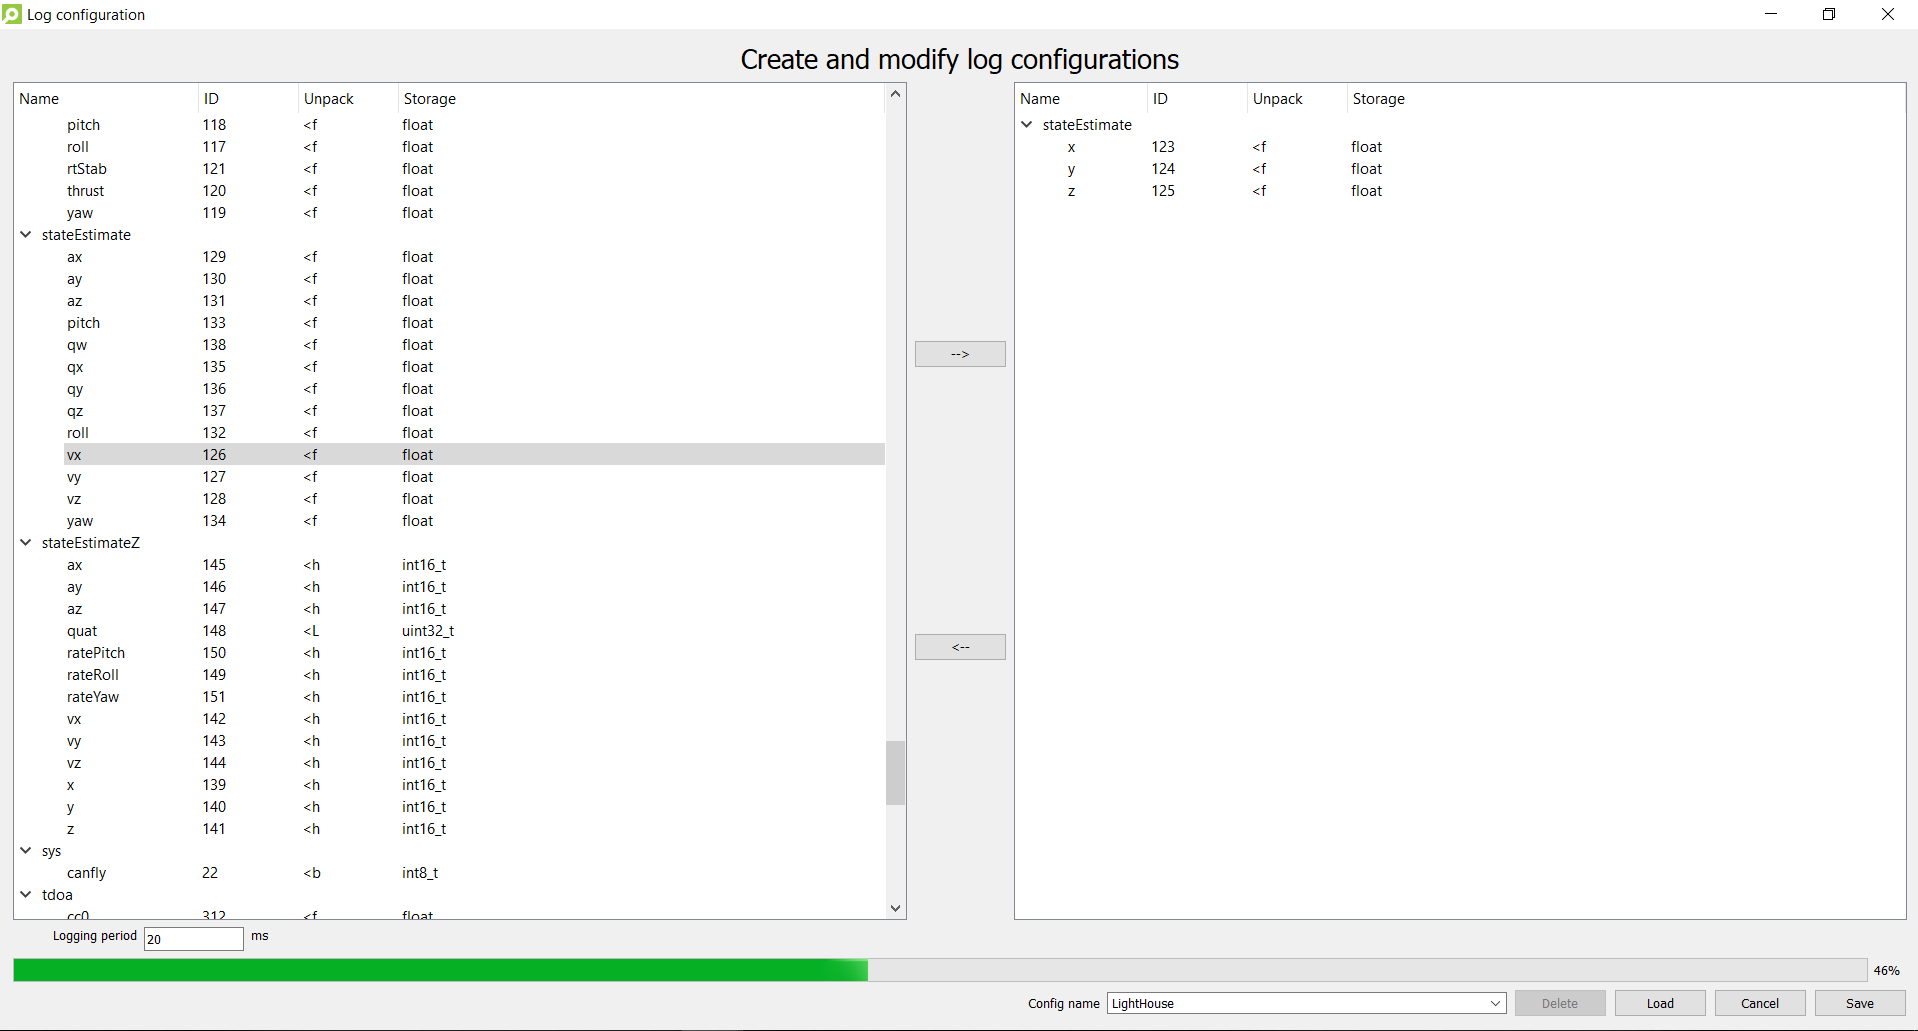
\includegraphics{images/logSetup.png}
\caption{Log Setup}
\end{figure}

The new log block should now be visible in the plotter tab of the
client. (Go to View -\textgreater{} Tabs if the plotter tab isn't
available)

\begin{figure}
\centering
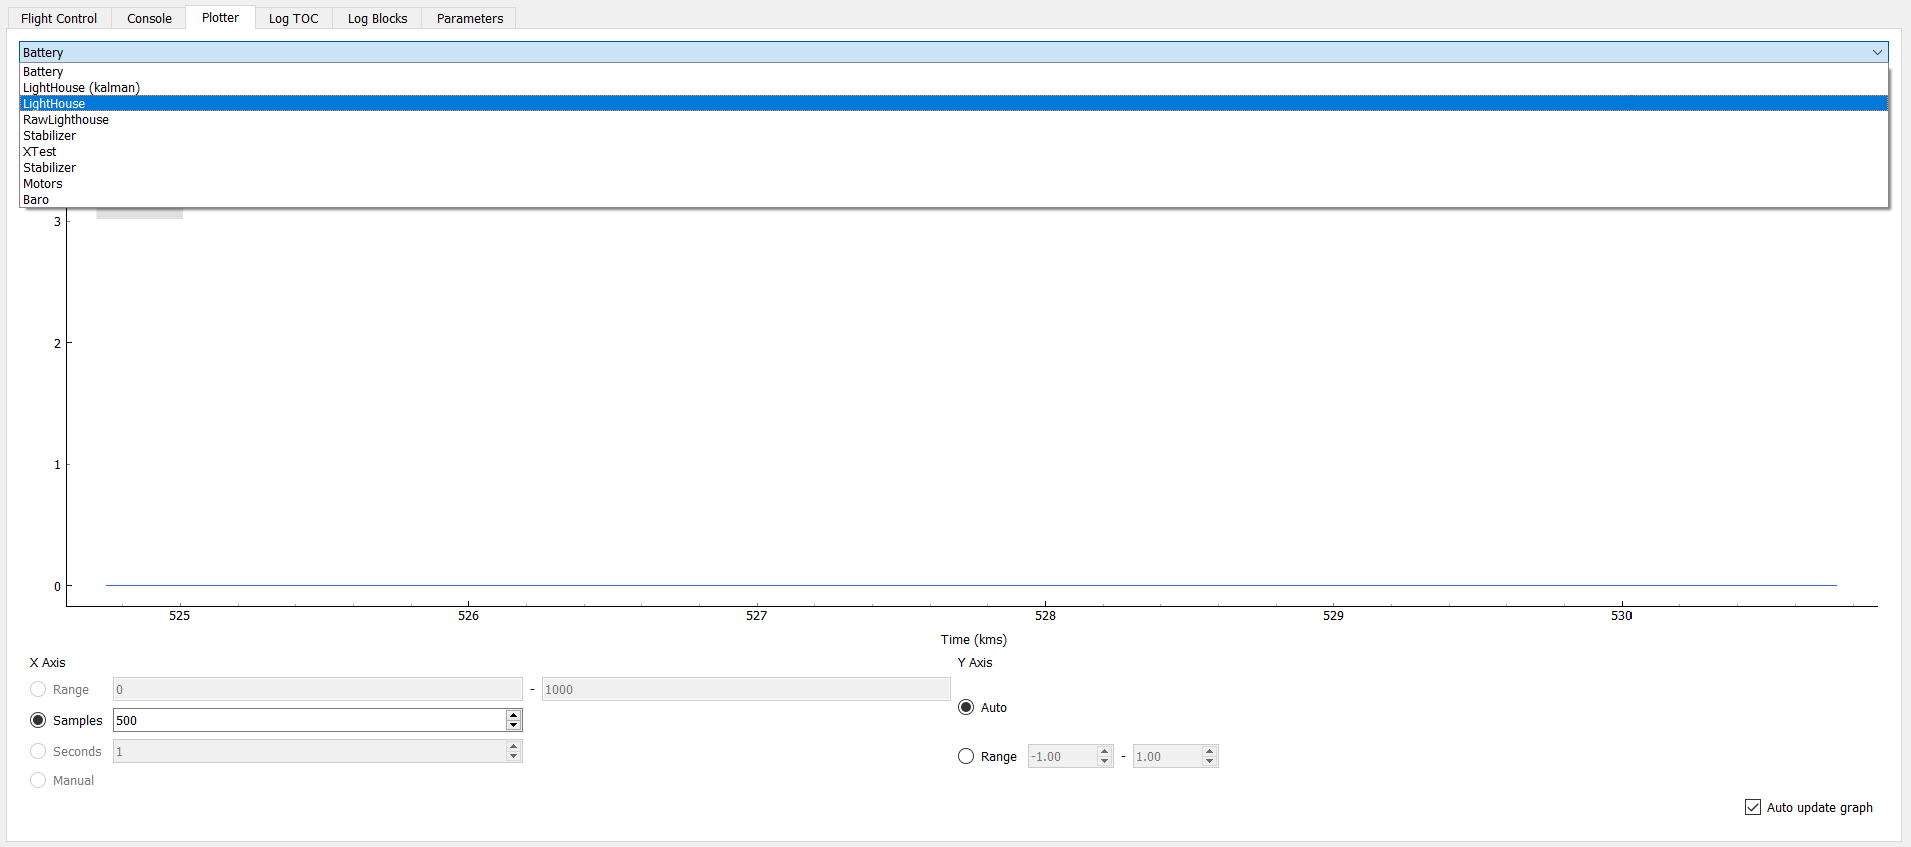
\includegraphics{images/plotterMenu.png}
\caption{Plotter Menu}
\end{figure}

The position of the drone should now be plotted to the screen, try
moving it around to check that the readings make sense.

\begin{figure}
\centering
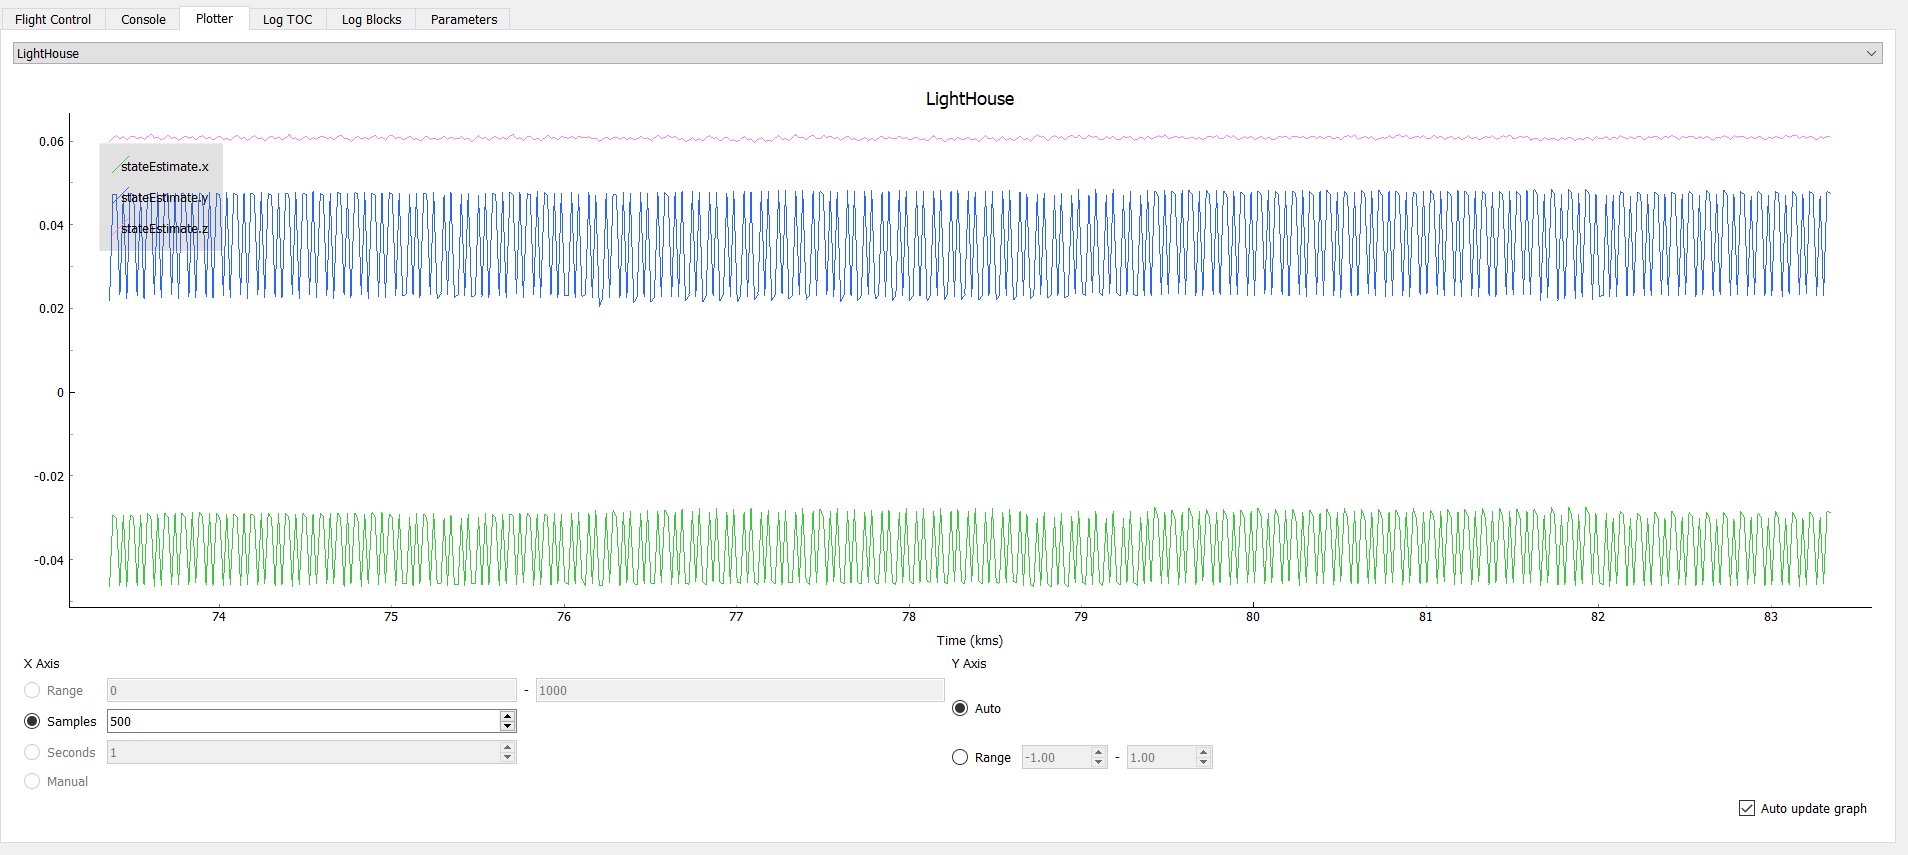
\includegraphics{images/plotterExample.png}
\caption{Plotter Example}
\end{figure}

\hypertarget{flight-assist.}{%
\subsubsection{Flight assist.}\label{flight-assist.}}

Place the crazyflie back inside of the play space. On the crazyflie
client, set the assist mode to position hold. You need a gamepad (x-box
controller) to fly the drone using the pc client.

The client supports multiple types of controllers, to select the correct
mapping select the Input device -\textgreater{} Device menu, or
Configure device mapping to create your own.

Here are the controls to fly a drone in position hold mode. Note 2
important things. 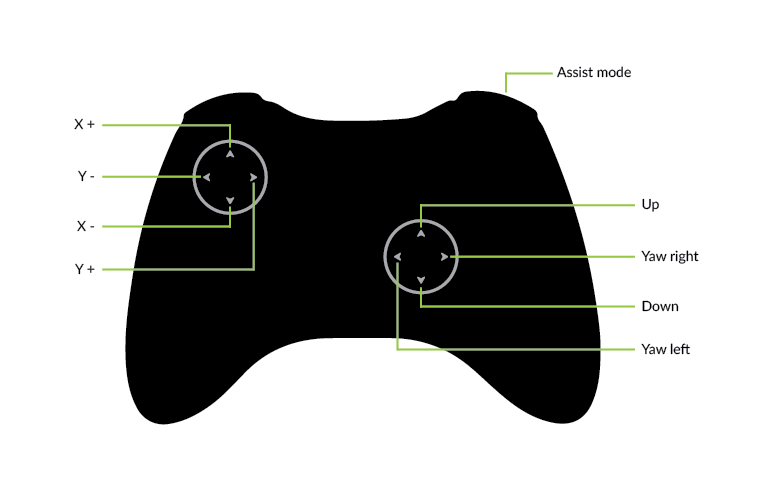
\includegraphics{images/controls.png}

\begin{enumerate}
\def\labelenumi{\arabic{enumi}.}
\tightlist
\item
  The controls are absolute and not relative to the direction that the
  drone is facing. Pushing the thust stick up will move the drone in the
  positive X no matter what the yaw is
\item
  The drone will only hold it's position if the assist mode button is
  held down, which is the right bumper on the Xbox controller. Note that
  these buttons are often the first ones to detereiorate on an Xbox
  controller, so if it is not working, you may need to re-map the assist
  button or press the bumper with more force than you might think.
\end{enumerate}

Start flight by holding down the assist button, the drone, without any
other inputs should try to hover itself very slightly above the ground.
If it does, move it up off the ground using the right stick. The drone
should hover in the same position as long as you hold down the assist
button.

The drone may drift slightly. This issue is generally fixed by
restarting the drone and ensuring that it is on a truly flat surface
when it is trying to stabalise itself.

The position hold is not likely going to be perfect.

If this works, it's worth trying out (almost) autonomous flight

\hypertarget{semi-autonomous-flight-openvr-grab-sample}{%
\subsubsection{Semi autonomous flight, openvr grab
sample}\label{semi-autonomous-flight-openvr-grab-sample}}

You will have to run this on a computer with Steam VR installed and
running.

Clone the repo for cflib, which allows autonomous flying

\begin{verbatim}
https://github.com/bitcraze/crazyflie-lib-python
\end{verbatim}

If you are on Linux, take note of the information in the README about
how to run these scripts without root, and install the package as per
the README.

Open up SteamVR, and make sure that all items except one controller are
visible within SteamVR (visible of the lighthouse deck) Place that one
controller on the floor next to the crazyflie drone, about 20cm away.

Before doing this, be ready to press Ctrl+C on the python script to
ensure that you can stop the drone if it behaves strangely.

Turn the crazyflie on inside the space, and run the following:

\begin{verbatim}
python examples/lighthouse/lighthouse_openvr_grab.py
\end{verbatim}

The drone should hover itself about 30cm above the controller. Take the
controller and use the trigger on the back to drag the drone around. To
stop it from flying, bring it close to the ground and exit the script
with Ctrl+C or similar.

\hypertarget{fully-autonomous-flight-light-grafitti-pathfinding-example.}{%
\subsubsection{Fully autonomous flight, light grafitti pathfinding
example.}\label{fully-autonomous-flight-light-grafitti-pathfinding-example.}}

Finally, this uses the code that we developed based off the grab system
that controls the drone to create a path.

First, open up a 3D modelling program such as Blender, and create a path
(a line of vertices, or a closed shape but curves also work). Keep in
mind that 1 unit in your software is equal to one meter of space, so
ensure that you are not flying too far in any particular direction, or
underneath the earth (below z=0).

Export your file as a .obj file. Then put it in the same directory as
this project

with the crazyflie radio attached, and cflib installed, run

\begin{verbatim}
python pathfind.py <exported_obj_file>
\end{verbatim}

Wait, and it should follow the path slowly. If the LED deck is installed
it will light up when it is following your path and turn off when it is
not. It should safely fly itself up and down.
